% BAI506 mini-project report, P2 component -- department house style as used for the proposal:
% Times New Roman 12 pt body, 1.5 spacing, bold 16/14 pt headings, header = title (left),
% footer = Dept of AI & ML, BMSIT&M / year / page. Swap the cover block for the official
% template page if the department issues one.
\documentclass[12pt,a4paper]{report}
\usepackage[utf8]{inputenc}
\usepackage[T1]{fontenc}
\usepackage{newtxtext,newtxmath}
\usepackage[margin=25mm,top=28mm,bottom=25mm]{geometry}
\usepackage{setspace}\onehalfspacing
\usepackage{booktabs,array,tabularx,longtable}
\usepackage{graphicx}
\usepackage{fancyhdr}
\usepackage{titlesec}
\usepackage{enumitem}
\usepackage{caption}
\usepackage[hidelinks]{hyperref}
\usepackage[table]{xcolor}
\usepackage{microtype}

% ---- fill these in -----------------------------------------------------------
\newcommand{\ProjectTitle}{Explainable Tuberculosis Screening from Chest X-Rays with Lesion Localisation for Triage in Resource-Limited Settings}
\newcommand{\ShortTitle}{Explainable Tuberculosis Screening from Chest X-Rays with Lesion Localisation}
\newcommand{\GuideName}{}
\newcommand{\SectionBatch}{}
\newcommand{\SubmissionDate}{November 2026}
\newcommand{\StudentOne}{}\newcommand{\USNOne}{}
\newcommand{\StudentTwo}{Atul Dhull}\newcommand{\USNTwo}{}
\newcommand{\StudentThree}{}\newcommand{\USNThree}{}
\newcommand{\StudentFour}{}\newcommand{\USNFour}{}
% ---------------------------------------------------------------------------

\titleformat{\chapter}[hang]{\bfseries\fontsize{16}{20}\selectfont}{\thechapter.}{0.6em}{}
\titlespacing*{\chapter}{0pt}{0pt}{14pt}
\titleformat{\section}{\bfseries\fontsize{14}{18}\selectfont}{\thesection}{0.6em}{}
\titleformat{\subsection}{\bfseries\fontsize{12}{15}\selectfont}{\thesubsection}{0.6em}{}
\pagestyle{fancy}\fancyhf{}
\fancyhead[L]{\small\ShortTitle}
\fancyfoot[L]{\small Dept of AI \& ML, BMSIT\&M}\fancyfoot[C]{\small 2026--27}\fancyfoot[R]{\small Page \thepage}
\renewcommand{\headrulewidth}{0.4pt}
\captionsetup{font=small,labelfont=bf}
\newcolumntype{L}{>{\raggedright\arraybackslash}X}
\newcommand{\ci}[2]{[$#1$, $#2$]}
\newcommand{\code}[1]{\texttt{#1}}
\setlength{\parskip}{4pt}

\begin{document}

% ================================================================ cover
\thispagestyle{empty}
\begin{center}
{\large\bfseries \textcolor[HTML]{C00000}{BMS} INSTITUTE OF TECHNOLOGY AND MANAGEMENT}\\[2pt]
{\small (An Autonomous Institute affiliated to VTU, Belagavi, Approved by AICTE New Delhi)}\\
{\small Yelahanka, Bengaluru 560064}\\[6pt]
{\bfseries Department of Artificial Intelligence and Machine Learning}\\[8pt]
\IfFileExists{logo.png}{
\includegraphics[width=26mm]{logo.png}}{}\\[8pt]
{\bfseries Mini Project Report -- BAI506}\\
{Academic Year 2026--27}\\[10pt]
\begin{tabular}{|p{0.22\textwidth}|p{0.42\textwidth}|p{0.26\textwidth}|}\hline
Section and Batch No:\newline\SectionBatch & Guide Name:\newline\GuideName & Submission Date:\newline\SubmissionDate\\[14pt]\hline
\end{tabular}\\[10pt]
\begin{tabular}{|p{0.94\textwidth}|}\hline
Mini Project Title\\\hline
\rule{0pt}{14pt}\bfseries\ProjectTitle\\[4pt]\hline
\end{tabular}\\[10pt]
\begin{tabular}{|p{0.11\textwidth}|p{0.30\textwidth}|p{0.51\textwidth}|}\hline
\cellcolor[HTML]{E8E8E8}Sl No & \cellcolor[HTML]{E8E8E8}USN & \cellcolor[HTML]{E8E8E8}Name\\\hline
1 & \USNOne & \StudentOne\\\hline 2 & \USNTwo & \StudentTwo\\\hline 3 & \USNThree & \StudentThree\\\hline 4 & \USNFour & \StudentFour\\\hline
\end{tabular}\\[10pt]
\begin{tabular}{|p{0.43\textwidth}|p{0.51\textwidth}|}\hline
Project Category & Computer Vision -- medical imaging (P2 component report: classifier, evaluation and calibration)\\\hline
\end{tabular}\\[26pt]
\hfill Signature of Guide
\end{center}
\clearpage

% ================================================================ abstract
\chapter*{Abstract}
\addcontentsline{toc}{chapter}{Abstract}
Tuberculosis remains one of the deadliest infectious diseases, and India carries a quarter of the global burden. Chest radiography is the recommended first screening test, and since 2021 the WHO has endorsed computer-aided detection (CAD)~\cite{who2021} as an alternative to human reading for people aged 15 and above. Published CAD methods report above 0.99 AUROC on the public TBX11K benchmark. This project asked what survives when such a model is evaluated the way a screening programme would use it: on a programmatic active-case-finding cohort with a microbiological reference standard and a certified commercial reader scored on the same patients.

We built a classifier from a frozen radiology foundation model (RAD-DINO) and a 769-parameter regional head that takes the maximum over a $12\times12$ grid of region scores, so that the region which decides each image is known exactly. It reaches 0.9368 AUROC on TBX11K development and 0.7242 on the reserved half of a 2,708-participant Vietnamese screening cohort, against 0.7862 for Lunit INSIGHT CXR on the same patients. The loss concentrates in people with previous tuberculosis, reproducing a published effect. We then ran eleven pre-registered interventions. Evaluated against their declared decision criteria, several were negligible or adverse and one was positive but below the threshold on the primary split. Three---training to the active-TB label, a related encoder, and fusing a twelve-field screening questionnaire---improve the screening result and leave the benchmark unchanged, and they overlap rather than add. The best configuration reaches 0.7941 with the questionnaire, numerically above the comparator (0.7780) with a confidence interval that includes zero; a field ablation shows the margin above the comparator is a per-scanner adjustment, which unlabelled centering recovered (0.7795 with 25 images per scanner; paired $+0.0281$ \ci{+0.0074}{+0.0486} at 100) under the nominal sampling condition tested, and which fails a pre-registered stability bound when the calibration sample comes from a different population. The decision region of the head overlaps an annotated active-TB lesion in 95.9\% of 49 development images. A concept-probing instrument built on radiology-report text embeddings was shown to be negation-blind and its findings withdrawn.

On an exposed screening cohort the system reached a numerically higher AUROC point estimate than commercial CAD; the paired interval includes zero, so no superiority, equivalence or non-inferiority claim is supported. It has a measured low-memory inference footprint on a consumer laptop GPU, exact attribution and a measured localisation result, and the report states why no superiority claim is available from public data.
\clearpage
\tableofcontents
\clearpage

% ================================================================ 1
\chapter{Introduction}
\section{Background}
India accounts for roughly 25\% of the world's tuberculosis cases (WHO Global Tuberculosis Report 2025~\cite{who2025}). Radiologists are scarce relative to need and concentrated in cities, so chest X-rays from district hospitals and screening camps can wait days for a reading. CAD software can read a digital chest X-ray in seconds and is WHO-recommended as an alternative to human reading for screening and triage in people aged 15 and above, against a target product profile of 90\% sensitivity at 70\% specificity~\cite{who2021}.

\section{Problem statement}
As proposed: \emph{to develop an explainable computer-aided detection system that identifies tuberculosis on chest X-rays, distinguishes it from other lung abnormalities, localises the affected regions, and operates at a sensitivity and specificity suitable for triage in resource-limited screening settings.}

As implemented by this component: to develop a chest-X-ray-based tuberculosis screening system that estimates active-TB suspicion, provides region-level attribution, and supports referral decisions in resource-limited screening settings. The production classifier is trained on healthy versus tuberculosis images and is a screening classifier, not a differential-diagnosis model; distinguishing TB from other lung abnormalities was measured (Section~\ref{sec:ladder}) but is not what the classifier was built to do.

\section{Objectives as proposed, and how each stands}
\begin{tabularx}{\textwidth}{@{}LL@{}}\toprule
\textbf{proposed objective} & \textbf{outcome}\\\midrule
Classifier on TBX11K reaching $\geq 90\%$ sensitivity at $\geq 70\%$ specificity on a held-out internal split, with AUROC reported & The numerical target was achieved on the development subset (sensitivity 1.00 at 70\% specificity; AUROC 0.9368 regional head / 0.9949 global probe), \textbf{but this is not an independent held-out evaluation}: development data informed early stopping and threshold fitting, the split is provisional, and the internal-test partition was used only once in a rehearsal. \textbf{Not met on the screening cohort}: sensitivity 0.62 raw, 0.74 with questionnaire fusion, at 70\% specificity.\\
Three-class classifier (healthy / sick-non-TB / TB) & Measured against a binary head: no difference on the primary metric (0.9661 both). Binary adopted; the three-class output is auxiliary.\\
Evaluation on Shenzhen and Montgomery & Done: 0.9690 / 0.9690 (regional head). These are curated case-control sets and, as Chapter~4 shows, overstate screening performance by 0.2 AUROC.\\
TB-region detector and detection AP; TBX11K online challenge submission & Detector is P1/P3's component (not reported here). No challenge submission was made.\\
Web tool showing TB probability, lesion localisation and ranking; $< 2$\,s per image on a laptop GPU & Served: \code{/v2/batch} ranks a batch by a TB \textbf{screening score} (the image logit---not a probability: a sigmoid of it has expected calibration error 0.49 and calibration slope 0.30 on the Vietnam cohort, so the UI never shows one), with the $12\times12$ region map, the exact decision region and an overlay per case; triage screen at \code{/v2/ui}. \textbf{Met after the segmenter was moved to the GPU: median 0.13\,s/image end-to-end (p90 0.15\,s) on the laptop GPU, after a $\sim$40\,s first-call model load; masks agree with the training-time CPU masks at 99.998\% of pixels.} On CPU alone the pipeline is $\approx 2.1$\,s/image.\\\bottomrule
\end{tabularx}

\section{Scope of this report}
This is the P2 component report: it covers the classification and evaluation component in full and references the other components where they interact. If BAI506 requires a single complete team report, the P1 (data and splits), P3 (lesion detector) and P4 (sealed-evaluation machinery) components must be added before submission.

% ================================================================ 2
\chapter{Literature Survey}
\textbf{Benchmarks and architectures.} TBX11K~\cite{liu2024} is the largest public TB chest-X-ray benchmark (11,200 images with lesion boxes). Its authors' SymFormer reaches 99.1\% AUROC on the official test split. Shenzhen and Montgomery~\cite{jaeger2014} are the standard external sets. Published numbers on these are near saturation: in our own measurements ten preprocessing variants of one model all reach sensitivity 1.0 at 70\% specificity on TBX11K, so the benchmark cannot rank methods finely. General-purpose vision--language models reach about 0.80 zero-shot on TBX11K~\cite{akhtar2026}.

\textbf{Foundation models for chest X-rays.} RAD-DINO~\cite{perezgarcia2025} is a self-supervised ViT-B/14 trained on chest radiographs without text supervision; MAIRA-2 released a continuation trained on a larger corpus. XraySigLIP~\cite{xraysiglip} is an image--text model at 512\,px. Frozen encoders with light heads are established for TB: RADAR~\cite{rege2026} cross-attends a learned TB query over patches with adversarial domain objectives; CheXFound/GLoRI~\cite{yang2025} studies global-plus-local adaptation. We claim no architectural novelty over these.

\textbf{Real-world evaluation.} Codlin et al.~\cite{codlin2025} evaluated Lunit INSIGHT CXR versions on 2,708 participants of a Vietnamese active-case-finding programme with Xpert Ultra reference, and released the data; they report, as did Kagujje et al.~\cite{kagujje2023} and Qin et al.~\cite{qin2024}, that CAD accuracy falls in people with previous tuberculosis. Our work reproduces that effect rather than discovering it.

\textbf{Explainability.} Saliency and post-hoc heatmaps are the norm. Max-pooled multiple-instance heads make attribution exact by construction, which is the route taken here. Text-anchored concept probing through vision--language models (CLEAR~\cite{han2026}) was attempted and is reported as a negative result in Chapter~6.

\section{Limitations of the surveyed work}
Benchmark results are reported on curated case-control data with saturated metrics; external validation is usually on two small curated sets; previous-TB performance is rarely stratified; and commercial systems are evaluated mostly by their makers. None of the surveyed academic systems reports a head-to-head against a commercial reader on the same screening participants.

\section{Outcome of the survey}
Evaluate along a ladder from benchmark to screening cohort with a commercial comparator on identical patients; pre-register every intervention; make attribution exact rather than post-hoc; state what the evidence does not support.

% ================================================================ 3
\chapter{Data and Methodology}
\section{Datasets}
\begin{tabularx}{\textwidth}{@{}lLL@{}}\toprule
dataset & $n$ & role\\\midrule
TBX11K (core train/val lists) & 8,400 (800 TB; boxes labelled active or obsolete) & training and internal evaluation; re-split 5,941 / 659 / 899 / 901 (provisional C01)\\
Vietnam screening cohort (Dryad,~\cite{codlin2025}) & 2,708 (280 Xpert-positive; 36\% previous TB; three scanners; 12-field questionnaire; Lunit scores) & the programmatic screening cohort used for exploratory evaluation; split once into TUNE 1,352 and REPORT 1,356\\
Shenzhen, Montgomery & 662, 138 & curated external\\
TBX11K DA / DB & 72, 104 & curated external\\\bottomrule
\end{tabularx}

Training rows for the production head are the healthy and tuberculosis images of the train split (3,241; 541 positive). Sick-non-TB train images are excluded (Section~\ref{sec:ladder} discusses the consequence).

\section{Pipeline}
\begin{enumerate}[leftmargin=1.6em,itemsep=1pt]
\item \textbf{Standardise}: greyscale, resize to 512\,px (DICOM: VOI LUT, 0.5/99.5 percentile clip).
\item \textbf{Quality gate}: a rule-based check that rejects undecodable or implausible inputs; a rejected image never carries a score.
\item \textbf{Lung mask}: a public PSPNet segmenter on the GPU; pixels outside the lungs are set to the image mean. This removes a border-reading shortcut quantified in Chapter~4.
\item \textbf{Encode}: frozen RAD-DINO ViT-B/14 at 518\,px; the $37\times37$ patch tokens are average-pooled to a $12\times12$ grid of 768-d region vectors, each L2-normalised.
\item \textbf{Head}: one $\mathrm{Linear}(768\to1)$ applied to every region; the image logit is the \textbf{maximum} over the 144 region logits. Five seeds are averaged.
\item \textbf{Operating points}: thresholds at 0.70 and 0.90 specificity, fitted on TBX11K development only.
\item \textbf{Optional fusion}: logistic regression on the standardised image score plus twelve questionnaire and scanner fields.
\end{enumerate}
Training: AdamW $3\mathrm{e}{-3}$, batch 256, weight decay $10^{-4}$, logit adjustment by the training prior, early stopping on development AUROC with patience 15, seeds 17/29/43/61/79. Trainable parameters: 769 per seed (3,845 total) plus 13 for fusion; frozen: 86,580,480.

\subsection{Baseline versus research candidate v3}
\begin{tabularx}{\textwidth}{@{}lLL@{}}\toprule
component & baseline & research candidate v3\\\midrule
encoder (frozen) & \code{microsoft/rad-dino} @ \code{110cbc18\ldots} & \code{microsoft/rad-dino-maira-2} @ \code{a6132efb\ldots} (same ViT-B/14 architecture, continued self-supervised training)\\
training target & \code{tb\_label}: active, latent and mixed TB positive; healthy negative & \code{active\_tb\_label}: active and mixed TB positive; latent (obsolete-only) TB \textbf{relabelled negative} alongside healthy\\
training rows & 3,241 (541 positive) & 3,241 (447 positive)\\
region aggregation & $12\times12$ maximum & $12\times12$ maximum\\
head & $\mathrm{Linear}(768\to1)$, 769 parameters per seed, 5 seeds & identical\\
clinical fusion & optional, 12 fields & optional, 12 fields including two scanner indicators\\
status & served default (bundle v2) & frozen research candidate (bundle v3), not promoted\\\bottomrule
\end{tabularx}

\section{Evaluation protocol}
Every experiment after the headline result was pre-registered: a protocol file hashed before any fitting, a primary evaluation split that the intervention was not designed on (TBX11K calibration, 899 images, 81 active-TB positives), a minimum meaningful effect of $+0.02$ AUROC with a paired-bootstrap interval excluding zero, and a reproduction gate requiring the production arm to be reproduced to within 0.0005 before any contrast is read. The screening tuning half is reported as context and is exposed (Chapter~7). Interventions that act on cohort-specific quantities (scanner subspace, aggregator selection, local-site refit, questionnaire fusion, per-scanner centering) have no calibration endpoint by design and are exploratory on the screening cohort. Bootstrap resampling is at the participant level; the released data carry no screening-event identifier, so clustering within the 127 screening events is not modelled and intervals may understate uncertainty. TBX11K's internal-test partition and the Vietnam REPORT half were not read for any of the interventions.

\section{Software architecture}
\begin{figure}[h]\centering
\begin{minipage}{0.95\textwidth}\small\ttfamily
image (any size) -> standardise 512x512 -> quality gate -> reject | pass\\
\hspace*{1em}-> lung mask (PSPNet, GPU; outside-lung -> image mean)\\
\hspace*{1em}-> frozen encoder (ViT-B/14 @ 518 px) -> 37x37 tokens -> pool -> 12x12 x 768-d, L2\\
\hspace*{1em}-> Linear(768->1) per region, 5 seeds -> max over 144 regions -> image logit\\
\hspace*{1em}-> operating points (dev-fitted) -> optional fusion (12 fields, exploratory)\\
served by scripts/serve\_v2.py: /v2/analyse, /v2/batch (ranked), /v2/overlay, /v2/ui, /v2/calibration/propose
\end{minipage}
\caption{The served pipeline. The arg-max region is the decision region exactly.}
\end{figure}

% ================================================================ 4
\chapter{Results I: the Ladder from Benchmark to Clinic}\label{sec:ladder}
\section{The benchmark figure is partly a shortcut}
A global linear probe on the frozen encoder reaches 0.9949 on TBX11K development---and 0.9094 from the \textbf{outer 12\% of the image alone}, a frame containing no lung. The shortcut is dataset-specific: the border-only model scores 0.52--0.62 at the four external sites, while a lungs-only model tracks the full image within 0.015 everywhere. The production model is therefore lung-masked.

\section{Performance along the ladder}
\begin{center}\begin{tabular}{@{}llcc@{}}\toprule
rung & cohort & regional $12\times12$ max & comparator\\\midrule
benchmark & TBX11K development (659) & 0.9368 & ---\\
curated external & Shenzhen / Montgomery & 0.9690 / 0.9690 & ---\\
curated external & DA / DB & 0.9755 / 0.9497 & ---\\
\textbf{screening} & \textbf{Vietnam REPORT (1,356)} & \textbf{0.7242} \ci{0.6843}{0.7618} & \textbf{0.7862}\\\bottomrule
\end{tabular}\end{center}
The aggregator matters: \code{mean} over the same regions (mathematically global pooling) stays at 0.636--0.642 on the tuning half while \code{max} reaches 0.7239; learned gated attention is worse (0.6416). Selection optimism between tuning and reporting halves is $-0.0005$.

The screening loss is a negative-class problem. TB-versus-healthy on TBX11K is AUROC 1.0000; a screening queue's Xpert-negatives include healed TB and chronic lung disease, and the model learned abnormality. A distance-based out-of-distribution gate does not see this: the screening cohort sits at the same embedding distance as Shenzhen and the gate passes 99.2\% of it.

\section{Where the loss is: previous tuberculosis}
Under the construction used in the published literature, our AUROC is 0.7720 in participants without previous TB and \textbf{0.6392} with it (degradation $+0.1328$ \ci{0.0718}{0.1951}). The comparator degrades from 0.8170 to 0.7192. The difference in differences, $+0.0481$ \ci{-0.0170}{+0.1113}, includes zero: we cannot claim to degrade more than the comparator. Scanner appearance is not the cause: removing the scanner-predictive subspace from the embedding changes AUROC by $-0.0002$.

% ================================================================ 5
\chapter{Results II: Interventions}
\begin{tabularx}{\textwidth}{@{}r@{\hspace{0.5em}}Lp{0.2\textwidth}p{0.24\textwidth}p{0.14\textwidth}@{}}\toprule
\# & intervention & calibration $\Delta$ (primary) & screening $\Delta$ (context) & verdict\\\midrule
1 & scanner-subspace removal & --- & $-0.0002$ & null\\
2 & gated-attention aggregator & --- & $-0.082$ & worse\\
3 & \textbf{active-TB label} (latent $\to$ negative) & $-0.0037$ & \textbf{$+0.0203$ \ci{+0.0127}{+0.0279}} & external only\\
4 & head refit on local labels vs threshold only & 0 of 30 helped & --- & null\\
5 & lesion-box region supervision & $+0.0019$ \ci{-0.0019}{+0.0061} & $-0.0108$ & null\\
6 & \textbf{clinical-context fusion} & --- & \textbf{$+0.058$ \ci{+0.030}{+0.085}} & external only\\
7 & three training sources & $+0.0033$ \ci{+0.0006}{+0.0064} & $+0.0036$ & sub-threshold\\
8 & encoder ensemble & $+0.0006$ & $+0.011$ & null\\
9 & \textbf{MAIRA-2 encoder} & $-0.0004$ & \textbf{$+0.0188$ \ci{+0.0015}{+0.0364}} & external only\\
10 & levers 3 + 7 + 9 stacked & $-0.0010$ & $+0.0286$ (predicted $+0.047$) & not additive\\
11 & label-free scanner centering & --- & $+0.0281$ \ci{+0.0074}{+0.0486} ($n=100$) & worked under nominal sampling; fails stability bound\\\bottomrule
\end{tabularx}

\textbf{The three external levers overlap.} The best image-only head on the screening cohort is MAIRA-2 with the active label: 0.7585 \ci{0.722}{0.796}, $+0.0348$ over production, $-0.0032$ on calibration. Adding the extra sources on top subtracts. A 2,304-dimensional head on three concatenated encoders has the best development AUROC ever fitted (0.9505) and the worst transfer ($-0.0137$): more capacity learned the benchmark better and the clinic worse, which is why the backbone was never fine-tuned.

\textbf{Clinical-context fusion} (10-fold $\times$ 20 repeats, tuning half):
\begin{center}\begin{tabular}{@{}lccc@{}}\toprule
image score & raw & fused & previous TB raw $\to$ fused\\\midrule
production head & 0.7237 & 0.7809 & $0.6144 \to 0.7122$\\
MAIRA-2 + active head & 0.7585 & \textbf{0.7941} & $0.6501 \to 0.7349$\\
Lunit & 0.7780 & 0.7778 & $0.7062 \to 0.7144$\\\bottomrule
\end{tabular}\end{center}
Fused MAIRA-2 against the comparator's raw score: $+0.0170$ \ci{-0.0193}{+0.0527}---numerically above, not statistically. The comparator keeps the better AUPRC (0.328 vs 0.300). Sensitivity at 70\% specificity: 0.741 vs 0.708.

\textbf{What carries the fusion gain.} Leave-one-field-out: only the \textbf{scanner identifier} costs with an interval excluding zero ($-0.0138$; $-0.0429$ in previous TB). With the ten questionnaire fields alone the fused model is 0.7803 against the comparator's 0.7780, within noise. In particular, the previous-TB improvement in the fusion table above is carried mostly by the scanner term, not by the \code{past\_tb} field (removing it changes the previous-TB AUROC by $+0.004$): the questionnaire does not independently solve the previous-TB deficit. Scanner indicators produced a substantial improvement in our candidate ($\approx 0.02$ overall, 0.04 in previous TB), while adding the same fields to the comparator produced no material improvement in this experiment ($+0.001$). This does not independently establish scanner invariance in either system.

\textbf{Label-free scanner calibration.} Centering each scanner's scores on an unlabelled batch of its own images recovers the supervised gain---0.7795 with 25 images per scanner, and at 100 images a paired $+0.0281$ \ci{+0.0074}{+0.0486} (previous TB $+0.0557$) over the raw score---under the nominal sampling condition tested, and equalises referral burden across scanners (31\% / 24\% / 50\% $\to$ 40\% / 31\% / 32\%). It fails a pre-registered stability bound when the calibration batch is drawn from a different population: a previous-TB-only batch lowers that scanner's sensitivity by 0.122 (bound 0.10). The supervised term fails worse under the same shifts. The method is reported as not usable without a consecutive-sample guard, whose safety would have to be shown prospectively; a fail-closed proposal endpoint implements the guard and is labelled experimental.

\textbf{Cost.} Encoder 0.030\,s/image on a 6\,GB laptop GPU (peak 0.69\,GB), 1.25\,s on CPU; head fit 6.6\,s; full pipeline with the segmenter on the GPU: median 0.13\,s/image, p90 0.15\,s (masks identical to the CPU-built training cache at 99.998\% of pixels); $\approx 2.1$\,s/image on CPU. Threshold recalibration to a new site needs about 25 labelled local images.

% ================================================================ 6
\chapter{Explainability}
\section{Exact attribution, measured}
Because the image logit is the maximum over region logits, the arg-max region is the region that decided---no gradient, no post-hoc map. The attribution is exact at the $12\times12$ region level (cells of about 43\,px on a 512\,px image), not at pixel-level lesion boundaries. The unit of evaluation is the pooled $12\times12$ region cell: a cell overlaps a lesion box if its pixel footprint shares at least one 14-px ViT patch with the box after the exact preprocessing chain. On the 49 development images carrying an active-lesion box, the decision cell overlaps a box---a top-1 region-cell hit---in \textbf{95.9\%} \ci{89.8}{100} (top-3 cells: 100\%), against 36.7\% for a random lung cell, 18.4\% for a random cell and 8.2\% for the centre cell; the box-supervised head's top-1 region-cell hit rate on the same images is 0.939. This is ``the strongest region is on a lesion'', not lesion segmentation; it is exploratory on 49 curated images.

\begin{figure}[h]\centering
\IfFileExists{overlay_example.png}{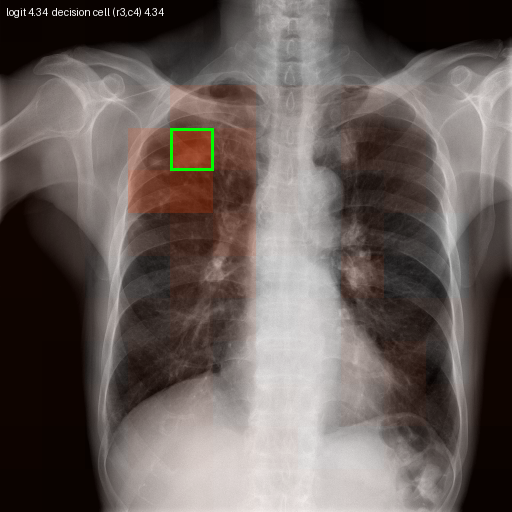
\includegraphics[width=0.5\textwidth]{overlay_example.png}}{\fbox{overlay example}}
\caption{Served overlay for a development active-TB image (logit 4.34): region logits shaded, the decision cell (row 3, column 4) boxed. Region-cell resolution, not a lesion boundary.}
\end{figure}

\section{A negative result on concept probing}
To ask what the score responds to, we correlated it with similarity to single-phrase text anchors through a public radiology vision--language model. \emph{Scarring} correlated at $\rho = 0.566$ with our score while carrying no information about TB (AUROC vs Xpert 0.494); \emph{consolidation} correlated negatively. A forensic pass showed the instrument cannot separate a finding from its negation: \emph{no scarring} correlates with the score at $+0.301$, the same sign as \emph{scarring}; \emph{no consolidation} at $-0.534$, more negative than \emph{consolidation}, because 27.6\% of vocabulary sentences about consolidation are negated normal-report language. All mechanistic readings from this instrument are withdrawn; the method limitation is reported instead.

% ================================================================ 7
\chapter{Limitations and What the Evidence Supports}
\begin{itemize}[leftmargin=1.4em,itemsep=1pt]
\item \textbf{Every screening number is on an exposed cohort.} The tuning half was used for selection by design; the reporting half, intended as read-once, was scored in six analyses, four of which influenced a decision. The three external levers were each found on the tuning half, so the fused 0.7941 is a best case designed on the cohort.
\item \textbf{The TBX11K split is provisional} and ships no patient identifier; 23 of 899 calibration images have a cross-split near-duplicate (effect 0.0003).
\item \textbf{No superiority, equivalence or non-inferiority is established} against the commercial comparator; the paired interval includes zero and the margin above the comparator is a scanner intercept.
\item \textbf{Confidence intervals are participant-level}; no screening-event identifier is released, so within-event clustering is not modelled.
\item \textbf{Scanner invariance is not demonstrated}; the label-free calibration is investigated, not validated.
\item \textbf{The localisation result} is on 49 development images; the lesion detector proper is another component.
\item HIV status was unavailable in every cohort.
\end{itemize}
What the evidence supports: \emph{on an exposed screening cohort, a frozen-encoder regional head with questionnaire fusion achieved a numerically higher AUROC point estimate than commercial CAD, with a paired interval that includes zero; without the scanner term the point estimate is 0.7803 against 0.7780; it runs on a consumer laptop GPU with a low memory footprint; its attribution is exact at region level and lands on annotated lesions in an exploratory test.}

% ================================================================ 8
\chapter{Conclusion and Future Scope}
A frozen radiology foundation model with a 769-parameter regional head reaches 0.94 on the benchmark and 0.72 on a screening cohort where commercial CAD reaches 0.79. Eleven pre-registered interventions found three levers that move the screening number and none that moves the benchmark; with a twelve-field screening questionnaire the system reaches a point estimate near the comparator's, and with a scanner-associated adjustment a point estimate above it, with paired intervals that include zero in both cases. The honest description is a scanner-aware screening research system with exact attribution, a measured localisation result, and an experimentally investigated label-free calibration mechanism---not a self-calibrating system and not a better one.

\textbf{Future scope.} (1) A head-to-head on a cohort nobody on the team has touched, with the frozen candidate and the comparator scored on the same patients and previous TB as a pre-specified subgroup; the protocol is pre-registered and hashed and a one-shot scorer exists. (2) A prospective test of the consecutive-sample guard for label-free calibration. (3) Documenting the benchmark's cross-split duplicates for the community.

% ================================================================ refs
\begin{thebibliography}{13}\small
\bibitem{liu2024} Y. Liu, Y.-H. Wu, S.-C. Zhang, L. Liu, M. Wu, M.-M. Cheng, ``Revisiting computer-aided tuberculosis diagnosis,'' \emph{IEEE Transactions on Pattern Analysis and Machine Intelligence} 46(4):2316--2332, 2024, doi:10.1109/TPAMI.2023.3330825.
\bibitem{jaeger2014} S. Jaeger et al., ``Two public chest X-ray datasets for computer-aided screening of pulmonary diseases,'' \emph{Quantitative Imaging in Medicine and Surgery} 4(6):475--477, 2014, doi:10.3978/j.issn.2223-4292.2014.11.20.
\bibitem{codlin2025} A. J. Codlin et al., ``Comparison of different Lunit INSIGHT CXR software versions when reading chest radiographs for tuberculosis,'' \emph{PLOS Digital Health} 4(4):e0000813, 2025, doi:10.1371/journal.pdig.0000813; data: Dryad doi:10.5061/dryad.5tb2rbpcv.
\bibitem{rege2026} A. A. Rege, A. M. Dukre, S. S. Shah, I. Razzak, ``RADAR: Acquisition-adversarial attention pooling over a frozen chest-radiograph foundation model for tuberculosis screening,'' in \emph{MICCAI 2026 Satellite Events --- TREAT-MMTB}, Springer proceedings (camera-ready, paper TREAT-MMTB\_012); code: github.com/adinathdukre/RADAR-TB.
\bibitem{yang2025} Z. Yang, X. Xu, J. Zhang, G. Wang, M. K. Kalra, P. Yan, ``Chest X-ray foundation model with global and local representations integration,'' \emph{IEEE Transactions on Medical Imaging} 44(12):4787--4799, 2025, doi:10.1109/TMI.2025.3581907.
\bibitem{kagujje2023} M. Kagujje, A. D. Kerkhoff, M. Nteeni, I. Dunn, K. Mateyo, M. Muyoyeta, ``The performance of computer-aided detection digital chest X-ray reading technologies for triage of active tuberculosis among persons with a history of previous tuberculosis,'' \emph{Clinical Infectious Diseases} 76(3):e894--e901, 2023, doi:10.1093/cid/ciac679.
\bibitem{qin2024} Z. Z. Qin et al., ``Computer-aided detection of tuberculosis from chest radiographs in a tuberculosis prevalence survey in South Africa: external validation and modelled impacts of commercially available artificial intelligence software,'' \emph{The Lancet Digital Health} 6(9):e605--e613, 2024, doi:10.1016/S2589-7500(24)00118-3.
\bibitem{perezgarcia2025} F. P\'erez-Garc\'ia et al., ``Exploring scalable medical image encoders beyond text supervision,'' \emph{Nature Machine Intelligence} 7:119--130, 2025, doi:10.1038/s42256-024-00965-w (RAD-DINO).
\bibitem{han2026} T. Han et al., ``CLEAR: an auditable foundation model for radiology grounded in clinical concepts,'' \emph{Nature Biomedical Engineering}, 2026, doi:10.1038/s41551-026-01741-4.
\bibitem{xraysiglip} Stanford AIMI, \emph{XraySigLIP (ViT-B/16, SigLIP, 512 px)}, Hugging Face model card, model id \code{StanfordAIMI/XraySigLIP\_\_vit-b-16-siglip-512\_\_webli}, revision \code{e2ad64ee}, accessed 2026-11-01 (the card cites Z. Chen et al., ``CheXagent: Towards a foundation model for chest X-ray interpretation,'' arXiv:2401.12208, 2024).
\bibitem{akhtar2026} M. Akhtar, M. Tanveer, M. Arshad, ``Beyond benchmark scores: Auditing medical vision-language models for chest X-ray tuberculosis screening,'' arXiv:2609.21763, 2026.
\bibitem{who2025} World Health Organization, \emph{Global Tuberculosis Report 2025}. Geneva: WHO, 2025.
\bibitem{who2021} World Health Organization, \emph{WHO consolidated guidelines on tuberculosis. Module 2: Screening --- systematic screening for tuberculosis disease}. Geneva: WHO, 2021.
\end{thebibliography}

\appendix
\chapter{Reproduction}
Every number traces to a run directory under \code{artifacts/} containing a hashed protocol, result tables, a test suite and a SHA-256 manifest; the project record indexes runs R1--R25:
\begin{center}\code{artifacts/P2\_PROJECT\_RECORD\_20261101.md}\end{center} The served system is \code{scripts/serve\_v2.py} (default bundle v2, RAD-DINO; \code{--bundle artifacts/p2/bundle\_v3\_candidate} selects the frozen research candidate); the triage screen is at \code{/v2/ui}. Unit tests: \code{py -3 -m pytest tests/ -q}.
\end{document}
